\documentclass{mcmthesis}
\mcmsetup{CTeX = false,    % 使用 CTeX 套装时,设置为 true
          tcn = {XXXXXX}, problem = \textcolor{red}{A},
          sheet = true, titleinsheet = true, keywordsinsheet = true,
          titlepage = false, abstract = true}
        
  %\usepackage{times}
  %\usepackage{newtxtext}
  %\usepackage{palatino}
  \usepackage{txfonts}
\usepackage[style=numeric,backend=biber,sorting=none,maxnames=3,minnames=1]{biblatex}
\addbibresource{reference.bib}

\usepackage{tocloft}
\setlength{\cftbeforesecskip}{6pt}
\renewcommand{\contentsname}{\hspace*{\fill}\Large\bfseries Contents \hspace*{\fill}}

\title{Here is the Title}
% \author{\small \href{http://www.latexstudio.net/}
%   {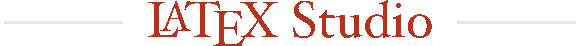
\includegraphics[width=7cm]{mcmthesis-logo}}}
\date{\today}

\begin{document}

\begin{abstract}

    A traditional bathtub cannot be reheated by itself, so users have to add hot
    water from time to time. Our goal is to establish a model of the temperature
    of bath water in space and time. Then we are expected to propose an optimal
    strategy for users to keep the temperature even and close to initial temperature
    and decrease water consumption.

    

    \begin{keywords}
        Heat transfer, Thermodynamic system, CFD, Energy conservation
    \end{keywords}

\end{abstract}

\maketitle

%% Generate the Table of Contents, if it's needed.
% \renewcommand{\contentsname}{\centering Contents}
\tableofcontents        % 若不想要目录, 注释掉该句
\thispagestyle{empty}

\newpage

\section{Introduction}

\subsection{Background}

Here is the background of the problem. The background of the problem is that

\subsection{Literature Review}

A traditional bathtub cannot be reheated by itself, so users have to add hot
water from time to time. Our goal is to establish a model of the temperature
of bath water in space and time. Then we are expected to propose an optimal
strategy for users to keep the temperature even and close to the initial
temperature and decrease water consumption. According to \textcite{kim2006},
He derived a relational equation based on the basic theory of heat transfer
to evaluate the performance of bath tubes. The major heat loss was found to be
due to evaporation. Moreover, he found out that the speed of heat loss depends
more on the humidity of the bathroom than the temperature of water contained
in the bathtub. So, it is best to maintain the temperature of bathtub water to
be between 41 to 45$^{\circ}$C and the humidity of bathroom to be 95\%.
Traditional bath systems have significant limitations in temperature control.
To address this, we introduce heat transfer formulas as
discussed (\cite[123]{holman2002}).

\subsection{Restatement of the Problem}

We are required to establish a model to determine the change of water temperature
in space and time. Then we are expected to propose the best strategy for the
person in the bathtub to keep the water temperature close to initial temperature
and even throughout the tub. Reduction of waste of water is also needed. In
addition, we have to consider the impact of different conditions on our model,
such as different shapes and volumes of the bathtub, etc.

In order to solve those problems, we will proceed as follows:

\begin{itemize}
    \item {\bf Stating assumptions}. By stating our assumptions, we will narrow the
          focus of our approach towards the problems and provide some insight into bathtub
          water temperature issues.

    \item {\bf Making notations}. We will give some notations which are important for
          us to clarify our models.

    \item {\bf Presenting our model}. In order to investigate the problem deeper, we
          divide our model into two sub-models. One is a steady convection heat transfer
          sub-model in which hot water is added constantly. The other one is an unsteady
          convection heat transfer sub-model where hot water is added discontinuously.



\end{itemize}

\section{Assumptions and Justification}

To simplify the problem and make it convenient for us to simulate real-life
conditions, we make the following basic assumptions, each of which is properly
justified.

\begin{itemize}
    \item {\bf The bath water is incompressible Non-Newtonian fluid}. The
          incompressible Non-Newtonian fluid is the basis of Navier–Stokes equations
          which are introduced to simulate the flow of bath water.

    \item {\bf All the physical properties of bath water, bathtub and air are
          assumed to be stable}. The change of those properties like specific heat,
          thermal conductivity and density is rather small according to some
          studies. It is complicated and unnecessary to consider these little
          change so we ignore them.


\end{itemize}

\section{Notations}

\begin{center}
    \begin{tabular}{clc}
        {\bf Symbols} & {\bf Description}                    & \quad {\bf Unit}        \\[0.25cm]
        $h$           & Convection heat transfer coefficient & \quad W/(m$^2 \cdot$ K)
        \\[0.2cm]
        $k$           & Thermal conductivity                 & \quad W/(m $\cdot$ K)   \\[0.2cm]
        $c_p$         & Specific heat                        & \quad J/(kg $\cdot$ K)  \\[0.2cm]
        $\rho$        & Density                              & \quad kg/m$^2$          \\[0.2cm]
        $\delta$      & Thickness                            & \quad m                 \\[0.2cm]
        $t$           & Temperature                          & \quad $^\circ$C, K      \\[0.2cm]
        $\tau$        & Time                                 & \quad s, min, h         \\[0.2cm]
        $q_m$         & Mass flow                            & \quad kg/s              \\[0.2cm]
        $\Phi$        & Heat transfer power                  & \quad W                 \\[0.2cm]
        $T$           & A period of time                     & \quad s, min, h         \\[0.2cm]
        $V$           & Volume                               & \quad m$^3$, L          \\[0.2cm]
        $M,\,m$       & Mass                                 & \quad kg                \\[0.2cm]
        $A$           & Aera                                 & \quad m$^2$             \\[0.2cm]
        $a,\,b,\,c$   & The size of a bathtub                & \quad m$^3$
    \end{tabular}
\end{center}

\noindent where we define the main parameters while specific value of those
parameters will be given later.

\section{Model Overview}

To simplify the modeling process, we firstly assume there is no person in the
bathtub. We regard the whole bathtub as a thermodynamic system and introduce
heat transfer formulas. We establish two sub-models: adding water constantly
and discontinuously. For the former sub-model, we define the mean temperature
of bath water and introduce Newton's cooling formula to determine the heat
transfer capacity. After deriving the value of parameters, we deduce formulas
to derive results and simulate the change of temperature field via CFD, as
described by \textcite{anderson2006}.

In our basic model, we aim at three goals: keeping the temperature as even as
possible, making it close to the initial temperature and decreasing the water
consumption.


\section{Sub-model I : Adding Water Continuously}

As for the second sub-model, we define an iteration consisting of two processes:
heating and standby. According to the energy conservation law, we obtain the
relationship of time and total heat dissipating capacity. Then we determine
the mass flow and the time of adding hot water. We also use CFD to simulate
the temperature field in the second sub-model, following the techniques
outlined by \textcite{website2024}.

We first establish the sub-model based on the condition that a person add water
continuously to reheat the bathing water. Then we use Computational Fluid
Dynamics (CFD) to simulate the change of water temperature in the bathtub. At
last, we evaluate the model with the criteria which have been defined before.

\subsection{Model Establishment}

Since we try to keep the temperature of the hot water in bathtub to be even,
we have to derive the amount of inflow water and the energy dissipated by the
hot water into the air.


\subsubsection{Control Equations and Boundary Conditions}

According to thermodynamics knowledge, we recall on basic convection
heat transfer control equations in rectangular coordinate system. Those
equations show the relationship of the temperature of the bathtub water in space.

We assume the hot water in the bathtub as a cube. Then we put it into a
rectangular coordinate system. The length, width, and height of it is $a,\, b$
and $c$.

\begin{figure}[h]
    \centering
    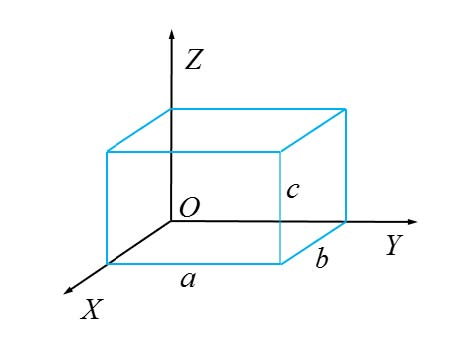
\includegraphics[width=8cm]{fig2.jpg}
    \caption{Modeling process} \label{fig2}
\end{figure}

In the basis of this, we introduce the following equations:

\begin{itemize}
    \item {\bf Continuity equation:}
\end{itemize}

\begin{equation} \label{eq1}
    \frac{\partial u}{\partial x} + \frac{\partial v}{\partial y} +
    \frac{\partial w}{\partial z} = 0
\end{equation}

\noindent where the first component is the change of fluid mass along the $X$-ray.
The second component is the change of fluid mass along the $Y$-ray. And the third
component is the change of fluid mass along the $Z$-ray. The sum of the change in
mass along those three directions is zero.

\begin{itemize}
    \item {\bf Moment differential equation (N-S equations):}
\end{itemize}

\begin{equation} \label{eq2}
    \left\{
    \begin{array}{l} \!\!
        \rho \Big(u \dfrac{\partial u}{\partial x} + v \dfrac{\partial u}{\partial y} +
        w\dfrac{\partial u}{\partial z} \Big) = -\dfrac{\partial p}{\partial x} +
        \eta \Big(\dfrac{\partial^2 u}{\partial x^2} + \dfrac{\partial^2 u}{\partial y^2} +
        \dfrac{\partial^2 u}{\partial z^2} \Big) \\[0.3cm]
        \rho \Big(u \dfrac{\partial v}{\partial x} + v \dfrac{\partial v}{\partial y} +
        w\dfrac{\partial v}{\partial z} \Big) = -\dfrac{\partial p}{\partial y} +
        \eta \Big(\dfrac{\partial^2 v}{\partial x^2} + \dfrac{\partial^2 v}{\partial y^2} +
        \dfrac{\partial^2 v}{\partial z^2} \Big) \\[0.3cm]
        \rho \Big(u \dfrac{\partial w}{\partial x} + v \dfrac{\partial w}{\partial y} +
        w\dfrac{\partial w}{\partial z} \Big) = -g-\dfrac{\partial p}{\partial z} +
        \eta \Big(\dfrac{\partial^2 w}{\partial x^2} + \dfrac{\partial^2 w}{\partial y^2} +
        \dfrac{\partial^2 w}{\partial z^2} \Big)
    \end{array}
    \right.
\end{equation}

\begin{itemize}
    \item {\bf Energy differential equation:}
\end{itemize}

\begin{equation} \label{eq3}
    \rho c_p \Big( u\frac{\partial t}{\partial x} + v\frac{\partial t}{\partial y} +
    w\frac{\partial t}{\partial z} \Big) = \lambda \Big(\frac{\partial^2 t}{\partial x^2} +
    \frac{\partial^2 t}{\partial y^2} + \frac{\partial^2 t}{\partial z^2} \Big)
\end{equation}

\noindent where the left three components are convection terms while the right
three components are conduction terms.

By Equation \eqref{eq3}, we have ......

......

On the right surface in Fig. \ref{fig2}, the water also transfers heat firstly
with bathtub inner surfaces and then the heat comes into air. The boundary
condition here is ......

\subsubsection{Definition of the Mean Temperature}

......

\subsubsection{Determination of Heat Transfer Capacity}

......


.....

\subsubsection{Calculating Results}

Putting the above value of parameters into the equations we derived before, we
can get the some data as follows:

%%普通表格
\begin{table}[h]  %h表示固定在当前位置
    \centering        %设置居中
    \caption{The calculating results}  %表标题
    \vspace{0.15cm}
    \label{tab2}                       %设置表的引用标签
    \begin{tabular}{|c|c|c|}  %3个c表示3列, |可选, 表示绘制各列间的竖线
        \hline                    %画横线
        Variables & Values & Unit  \\ \hline  %各列间用&隔开
        $A_1$     & 1.05   & $m^2$ \\ \hline
        $A_2$     & 2.24   & $m^2$ \\ \hline
        $\Phi_1$  & 189.00 & $W$   \\ \hline
        $\Phi_2$  & 43.47  & $W$   \\ \hline
        $\Phi$    & 232.47 & $W$   \\ \hline
        $q_m$     & 0.014  & $g/s$ \\ \hline
    \end{tabular}
\end{table}

From Table \ref{tab2}, ......

......

\section{Model Analysis and Sensitivity Analysis}

In consideration of evaporation, we correct the results of sub-models referring
to studies. We define two evaluation criteria
and compare the two sub-models. Adding water constantly is found to keep the
temperature of bath water even and avoid wasting too much water, so it is
recommended by us. We also conduct sensitivity analysis to determine the
influence of factors such as radiation heat transfer, the shape and volume of
the tub, the shape/volume/temperature/motions of the person, and the bubbles
made from bubble bath additives, as discussed
in (\cite{evaporation2018}; \cite{thesis2015}).

\subsection{The Influence of Different Bathtubs}

Definitely, the difference in shape and volume of the tub affects the
convection heat transfer. Examining the relationship between them can help
people choose optimal bathtubs.

\subsubsection{Different Volumes of Bathtubs}

In reality, a cup of water will be cooled down rapidly. However, it takes quite
long time for a bucket of water to become cool. That is because their volume is
different and the specific heat of water is very large. So that the decrease of
temperature is not obvious if the volume of water is huge. That also explains
why it takes 45 min for 320 L water to be cooled by 1$^\circ$C.

In order to examine the influence of volume, we analyze our sub-models
by conducting sensitivity Analysis to them.

We assume the initial volume to be 280 L and change it by $\pm 5$\%, $\pm 8$\%,
$\pm 12$\% and $\pm 15$\%. With the aid of sub-models we established before, the
variation of some parameters turns out to be as follows

%%三线表
\begin{table}[h] %h表示固定在当前位置
    \centering  %设置居中
    \caption{Variation of some parameters}  %表标题
    \label{tab7} %设置表的引用标签
    \begin{tabular}{ccccccc} %7个c表示7列, c表示每列居中对齐, 还有l和r可选
        \toprule  %画顶端横线
        $V$      & $A_1$   & $A_2$   & $T_2$    & $q_{m1}$ & $q_{m2}$ & $\Phi_q$ \\
        \midrule  %画中间横线
        -15.00\% & -5.06\% & -9.31\% & -12.67\% & -2.67\%  & -14.14\% & -5.80\%  \\
        -12.00\% & -4.04\% & -7.43\% & -10.09\% & -2.13\%  & -11.31\% & -4.63\%  \\
        -8.00\%  & -2.68\% & -4.94\% & -6.68\%  & -1.41\%  & -7.54\%  & -3.07\%  \\
        -8.00\%  & -2.68\% & -4.94\% & -6.68\%  & -1.41\%  & -7.54\%  & -3.07\%  \\
        -8.00\%  & -2.68\% & -4.94\% & -6.68\%  & -1.41\%  & -7.54\%  & -3.07\%  \\
        \bottomrule  %画底部横线
    \end{tabular}
\end{table}

\section{Strength and Weakness}

\subsection{Strength}

\begin{itemize}
    \item We analyze the problem based on thermodynamic formulas and laws, so that
          the model we established is of great validity.

    \item Our model is fairly robust due to our careful corrections in consideration
          of real-life situations and detailed sensitivity analysis.

    \item Via Fluent software, we simulate the time field of different areas
          throughout the bathtub. The outcome is vivid for us to understand the changing
          process.

\end{itemize}

\subsection{Weakness}

\begin{itemize}
    \item Having knowing the range of some parameters from others’ essays, we choose
          a value from them to apply in our model. Those values may not be reasonable in
          reality.

    \item Although we investigate a lot in the influence of personal motions, they
          are so complicated that need to be studied further.

    \item Limited to time, we do not conduct sensitivity analysis for the influence
          of personal surface area.
\end{itemize}

\section{Further Discussion}

Based on our model analysis and conclusions, we propose the optimal strategy
for the user in a bathtub and explain the reason for the uneven temperature
throughout the bathtub. In addition, we make improvements for applying our
model in real life, as suggested by the patent \textcite{patent2023}.

\printbibliography

\newpage

\begin{letter}{Dear, Mr. Alpha Chiang}

    In addition, your report must include a letter to the Chief Financial Officer
    (CFO) of the Goodgrant Foundation, Mr. Alpha Chiang, that describes the optimal
    investment strategy, your modeling approach and major results, and a brief
    discussion of your proposed concept of a return-on-investment (ROI). This letter
    should be no more than two pages in length.

    \vspace{\parskip}

    Sincerely yours,

    Your friends

\end{letter}

\newpage

\begin{appendices}

    \section{First appendix}

    Here are simulation programmes we used in our model as follow .\\

    \textbf{\textcolor[rgb]{0.98,0.00,0.00}{Input matlab source:}}
    \lstinputlisting[language=Matlab]{./code/mcmthesis-matlab1.m}

    \section{Second appendix}

    some more text \textcolor[rgb]{0.98,0.00,0.00}{\textbf{Input C++ source:}}
    \lstinputlisting[language=C++]{./code/mcmthesis-sudoku.cpp}

\end{appendices}

\AImatter

\begin{ReportAiUse}{9}
  \bibitem{AI1}
  Bing AI\\
  Query1: write a sort algorithm\\
  Output: Sure, I can help you with that. Here is a simple implementation of the selection sort algorithm in Python:
  \begin{lstlisting}[language=python]
def selection_sort(arr):
    for i in range(len(arr)):
        min_idx = i
        for j in range(i + 1, len(arr)):
            if arr[min_idx] > arr[j]:
                min_idx = j
        arr[i], arr[min_idx] = arr[min_idx], arr[i]
    return arr
\end{lstlisting}
  This algorithm sorts an array by repeatedly finding the minimum element from the unsorted part of the array and putting it at the beginning. \href{https://www.geeksforgeeks.org/sorting-algorithms/}{The time complexity of this algorithm is O($n^2$)}.

  There are many other sorting algorithms available such as bubble sort, insertion sort, merge sort, quick sort, heap sort, and more. Each of these algorithms has its own advantages and disadvantages. You can learn more about them on GeeksforGeeks and Programiz.

  I hope this helps!

  \bibitem{AI2}
  OpenAl Enie (Nov 5, 2023 version, Ernie 4.0)\\
  Query1: <insert the exact wording of any subsequent input into the Al tool>\\
  Output: <insert the complete output from the second query>

  \bibitem{AI3}
  Github CoPilot (Feb 3, 2024 version)\\
  Query1: <insert the exact wording you input into the Al tool>\\
  Output: <insert the complete output fron the Al tool>

  \bibitem{AI4}
  Google Bard (Feb 2,2024 version)\\
  Query: <insert the exact wording of your query>\\
  Output: <irsert the complete output from the Al tool>

  \bibitem{AI5}
  Bing AI\\
  Query: write a FFT algorithm\\
  Output: Sure, here is a Python implementation of the Fast Fourier Transform (FFT) algorithm:
  \begin{lstlisting}[language=python]
import numpy as np

def fft(x):
    n = len(x)
    if n == 1:
        return x
    even = fft(x[0::2])
    odd = fft(x[1::2])
    T = [np.exp(-2j * np.pi * k / n) * odd[k] for k in range(n // 2)]
    return [even[k] + T[k] for k in range(n // 2)] + [even[k] - T[k] for k in range(n // 2)]
\end{lstlisting}
  The FFT is a widely used algorithm for computing the \textbf{Discrete Fourier Transform (DFT)} of a sequence. It reduces the number of computations needed from O(n$^2$) to O(n log n) 12. The basic idea of the FFT is to apply divide and conquer. We divide the coefficient vector of the polynomial into two vectors, recursively compute the DFT for each of them, and combine the results to compute the DFT of the complete polynomial 3.

  I hope this helps!

\end{ReportAiUse}

\end{document}
%%
%% This work consists of these files mcmthesis.dtx,
%%                                   figures/ and
%%                                   code/,
%% and the derived files             mcmthesis.cls,
%%                                   mcmthesis-demo.tex,
%%                                   README,
%%                                   LICENSE,
%%                                   mcmthesis.pdf and
%%                                   mcmthesis-demo.pdf.
%%
%% End of file `mcmthesis-demo.tex'.
